\documentclass[10pt,aspectratio=169,american]{beamer}

\usepackage{unicode-math}
\defaultfontfeatures{Scale=MatchLowercase}
\defaultfontfeatures[\rmfamily]{Ligatures=TeX,Scale=1}
\usepackage{lmodern}
\usetheme{metropolis}
\usepackage{microtype}
\UseMicrotypeSet[protrusion]{basicmath}
\usepackage{parskip}
\usepackage{babel}
\usepackage{bookmark}
\usepackage{xurl}
\usepackage{listings}
\usepackage{lstlinebgrd}
% Match the paper's Inconsolata code font without changing the deck's body font.
\newfontfamily\paperCodeFont[Scale=1,BoldFont=Inconsolatazi4-Bold.otf]{Inconsolatazi4-Regular.otf}
\newsavebox{\programInvariantListing}
\newsavebox{\velvetIntroListing}

\definecolor{codeKeyword}{HTML}{204A87}
\definecolor{codeString}{HTML}{4E9A06}
\definecolor{codeOperator}{HTML}{CE5C00}
\definecolor{codeNumber}{HTML}{0000CF}
\definecolor{codeComment}{HTML}{8F5902}
\lstdefinestyle{paperLean}{
  basicstyle=\paperCodeFont\mdseries\color{black}\linespread{1}\fontsize{8.4}{9}\selectfont,
  columns=fullflexible,keepspaces=true,showstringspaces=false,
  frame=none,backgroundcolor=\color{white},
  aboveskip=0pt,belowskip=0pt,mathescape=true,
  alsoletter={_},
  morekeywords={def,method,return,require,ensures,do,let,mut,if,then,else,while,invariant,decreasing,fun,guard,by,prove_correct,loom_solve},
  keywordstyle=\color{codeKeyword}\bfseries,
  identifierstyle=\color{black}\mdseries,
  morestring={[b]"},stringstyle=\color{codeString}\mdseries,
  morecomment={[l]{--}},commentstyle=\color{codeComment}\mdseries\upshape,
  literate={:=}{{\textcolor{codeOperator}{:=}}}2
           {=>}{{\textcolor{codeOperator}{=>}}}2
           {:}{{\textcolor{codeOperator}{:}}}1
           {(}{{\textcolor{codeOperator}{(}}}1
           {)}{{\textcolor{codeOperator}{)}}}1
           {0}{{\textcolor{codeNumber}{0}}}1
           {1}{{\textcolor{codeNumber}{1}}}1
           {2}{{\textcolor{codeNumber}{2}}}1
           {3}{{\textcolor{codeNumber}{3}}}1
           {4}{{\textcolor{codeNumber}{4}}}1
           {5}{{\textcolor{codeNumber}{5}}}1
           {6}{{\textcolor{codeNumber}{6}}}1
           {7}{{\textcolor{codeNumber}{7}}}1
           {8}{{\textcolor{codeNumber}{8}}}1
           {9}{{\textcolor{codeNumber}{9}}}1
}

\urlstyle{same}
\setlength{\emergencystretch}{3em}

\usetikzlibrary{arrows,fit,backgrounds,calc,shapes.symbols}
% Small adjustments to the Metropolis theme used in ../par_incr_presentation.
\metroset{numbering=fraction,progressbar=frametitle}
\setbeamertemplate{navigation symbols}{}
\setbeamercolor{background canvas}{bg=white}

\newcommand{\AIImageCreditFrame}{-1}
\newcommand{\aiimagefooter}{%
  \xdef\AIImageCreditFrame{\number\value{framenumber}}%
}
\setbeamertemplate{frame footer}{%
  \ifnum\value{framenumber}=\AIImageCreditFrame\relax
    {\color{gray}Images are AI-generated}%
  \fi
}

% Eight authors and three affiliations need a more compact cover.
\setbeamerfont{title}{size=\Large}
\setbeamerfont{author}{size=\small,series=\bfseries}
\setbeamerfont{institute}{size=\scriptsize}
\setbeamerfont{date}{size=\small}

% The stock title page's fixed spacing is too tall for this author list at 16:9.
\setbeamertemplate{title page}{%
  \vspace*{2mm}
  
\includegraphics[height=9mm]{assets/nus-logo.png}%
  \hspace{8mm}%
  
\includegraphics[height=9mm]{assets/neapolis-logo.png}%
  \hspace{8mm}%
  \raisebox{1mm}{
\includegraphics[height=7mm]{assets/eth-logo.png}}\par
  \vspace{5mm}
  {\usebeamerfont{title}\usebeamercolor[fg]{title}\inserttitle\par}
  \vspace{2mm}
  \usebeamertemplate*{title separator}
  \vspace{3mm}
  {\usebeamerfont{author}\insertauthor\par}
  \vspace{2mm}
  {\usebeamerfont{institute}\insertinstitute\par}
  \vspace{3mm}
  {\usebeamerfont{date}\insertdate\par}
}

\pdfstringdefDisableCommands{%
  \def\textsuperscript#1{}%
  \def\underline#1{#1}%
  \def\\{ }%
}

% Keep the PDF metadata readable (without affiliation markers or TeX).
\hypersetup{
  pdftitle={Certified program synthesis with a multi-modal verifier},
  pdfauthor={Yueyang Feng, Dipesh Kafle, Vladimir Gladshtein, Vitaly Kurin, George Pîrlea, Qiyuan Zhao, Peter Müller, Ilya Sergey}
}


% Compact diagrams shared by the three invariant-validation slides.
\newcommand{\invariantFlow}[3]{%
\begin{center}
\begin{tikzpicture}[
  stage/.style={draw=teal!65,fill=teal!4,rounded corners=2pt,
    minimum width=36mm,minimum height=10mm,align=center,font=\small},
  flow/.style={->,thick,draw=mLightBrown}]
\node[stage] (a) at (0,0) {#1};
\node[stage] (b) at (4.7,0) {#2};
\node[stage] (c) at (9.4,0) {#3};
\draw[flow] (a) -- (b);
\draw[flow] (b) -- (c);
\end{tikzpicture}
\end{center}%
}
\lstdefinestyle{reviewJSON}{
  basicstyle=\paperCodeFont\mdseries\color{black}\linespread{1}\fontsize{7.7}{8.3}\selectfont,
  columns=fullflexible,keepspaces=true,showstringspaces=false,
  aboveskip=0pt,belowskip=0pt,mathescape=true,
  morestring={[b]"},stringstyle=\color{codeKeyword}\mdseries,
  morekeywords={false,true},keywordstyle=\color{codeOperator}\bfseries
}
\hypersetup{
  pdflang={en-US},
  colorlinks=true,
  linkcolor=teal,
  urlcolor=teal,
  pdfcreator={XeLaTeX / Beamer}
}

\title{Certified program synthesis\\
with a multi-modal verifier}
\author{Yueyang Feng\textsuperscript{1,*}, \underline{Dipesh Kafle}\textsuperscript{1,*},
Vladimir Gladshtein\textsuperscript{1}, Vitaly Kurin\textsuperscript{2}\\
George Pîrlea\textsuperscript{1}, Qiyuan Zhao\textsuperscript{1},
Peter Müller\textsuperscript{3}, Ilya Sergey\textsuperscript{1}}
\institute{\textsuperscript{1}National University of Singapore\quad
\textsuperscript{2}Neapolis University Pafos\quad
\textsuperscript{3}ETH Zurich\\[0.4em]
\textsuperscript{*}Joint first authors}
\date{ASE ’26 · October 15, 2026 · Munich, Germany}

\begin{document}

\begin{frame}
\titlepage
\end{frame}

\begin{frame}{Motivation}
\aiimagefooter
\centering
{\large AI writes code for us. An idea becomes an implementation in seconds.\par}
\vspace{1mm}

\includegraphics[width=0.86\textwidth,height=36mm,keepaspectratio]{assets/ai-code-review.png}

\pause

{\Large\bfseries\color{mLightBrown}Who reviews all this code?\par}
\vspace{1mm}
{\small Generating code is fast. Establishing confidence still takes tremendous amount of work.\par}

\end{frame}

\begin{frame}{Motivation}
\aiimagefooter
\begin{columns}[c,onlytextwidth]
\begin{column}{0.57\textwidth}
\centering

\includegraphics[width=\linewidth,height=33mm,keepaspectratio]{assets/ai-proof-checking.png}

{\large Ask the AI for a proof, too.\par}
\end{column}
\begin{column}{0.39\textwidth}
\small
\textbf{Fermat's Last Theorem}\\
13 million lines of Lean;\\
machine-checked proof.\\[-0.5mm]
{\scriptsize\href{https://www.anthropic.com/news/formalizing-fermats-last-theorem}{Anthropic, September 2026}}

\vspace{3mm}
\textbf{Navier--Stokes}\\
Proof released with a\\
Lean formalization.\\[-0.5mm]
{\scriptsize\href{https://openai.com/index/navier-stokes-solution/}{OpenAI, September 2026}}
\end{column}
\end{columns}

\vspace{4mm}
\centering
\textbf{Humans inspect the claim and its assumptions.}\\
The proof checker checks the derivation.

\end{frame}

\begin{frame}{Motivation}
\centering
{\large Can we automate the whole process?\par}
\vspace{4mm}

\begin{columns}[c,onlytextwidth]
\begin{column}{0.37\textwidth}
\centering
{\Large\bfseries English task\par}
\vspace{2mm}
Describe what the program should do.
\end{column}
\begin{column}{0.10\textwidth}
\centering
{\Huge\color{mLightBrown}$\longrightarrow$}
\end{column}
\begin{column}{0.47\textwidth}
\raggedright
{\large\bfseries Runnable program\par}
{\small An implementation we can execute.\par}
\vspace{2mm}
{\large\bfseries Formal specification\par}
{\small A precise statement of intended behavior.\par}
\vspace{2mm}
{\large\bfseries Checked proof\par}
{\small The program satisfies the specification.\par}
\end{column}
\end{columns}

\end{frame}

\begin{frame}{Why is this difficult?}
\setlength{\parskip}{0pt}
\textbf{\color{teal}Specifications are hard to get right}
\vspace{3mm}

Capturing intent precisely is difficult, even for humans.\\
We found issues in existing verification benchmarks:

\vspace{5mm}
\begin{columns}[c,onlytextwidth]
\begin{column}{0.47\textwidth}
\centering
{\Large\bfseries\color{mLightBrown}16 issues}\quad in \textbf{VERINA}
\end{column}
\begin{column}{0.47\textwidth}
\centering
{\Large\bfseries\color{mLightBrown}18 issues}\quad in \textbf{CLEVER}
\end{column}
\end{columns}

\vspace{8mm}
\uncover<2->{%
\textbf{\color{teal}Proofs are hard to complete}
\vspace{3mm}

Even for a correct program, proof search can consume many tokens\\
and still leave goals unproved.
}
\end{frame}

\begin{frame}{Easier, more efficient certified synthesis}
\begin{uncoverenv}<2->
\begin{columns}[T,onlytextwidth]
\begin{column}{0.30\textwidth}
\textbf{\color{teal}Test}

Reject incorrect candidates cheaply.
\end{column}
\begin{column}{0.30\textwidth}
\textbf{\color{teal}Automate}

Discharge goals with SMT and Lean automation like \texttt{grind}.
\end{column}
\begin{column}{0.30\textwidth}
\textbf{\color{teal}Prove interactively}

Handle goals automation cannot solve.
\end{column}
\end{columns}
\end{uncoverenv}

\vspace{8mm}
\uncover<3->{Combine \textbf{\textit{different modes}} to reject incorrect candidates and prove correct ones.\par}

\vspace{5mm}
\uncover<4->{\textbf{\color{mLightBrown}Our hypothesis:} Using \href{https://velvetprover.dev/}{\textbf{Velvet}}, a multi-modal verifier in Lean, we can certify more programs within the same budget.\par}

\end{frame}

\begin{frame}[fragile]{Velvet 101}
\setlength{\parskip}{0pt}
\begin{lrbox}{\velvetIntroListing}
\begin{minipage}{0.70\textwidth}
\begin{lstlisting}[
  style=paperLean,
  linebackgroundcolor={\color{white}\ifnum\value{lstnumber}=2 \color{blue!9}\fi\ifnum\value{lstnumber}>7 \ifnum\value{lstnumber}<10 \color{yellow!16}\fi\fi\ifnum\value{lstnumber}>14 \color{green!12}\fi},
  linebackgroundheight=6.8pt,linebackgrounddepth=2.2pt
]
method IsNonPrime (n : Nat) return (result : Bool)
  ensures result = true $\leftrightarrow$ $\neg$isPrime n
  do
    if n $\leq$ 1 then return true
    let mut i : Nat := 2
    let mut ret : Bool := false
    while i * i $\leq$ n
    invariant $\neg$ret $\leftrightarrow$ $\forall$d, 2 $\leq$ d $\land$ d < i $\to$ n % d $\neq$ 0
    invariant i $\geq$ 2 $\land$ (i - 1) * (i - 1) $\leq$ n
    do
      if n % i = 0 then ret := true
      i := i + 1
    return ret

prove_correct IsNonPrime by
  loom_solve  -- automated VC discharge
  ...         -- remaining interactive proof
\end{lstlisting}
\end{minipage}
\end{lrbox}
\begin{tikzpicture}
\node[inner sep=0pt,anchor=west] (velvetCode) at (0,0)
  {\usebox{\velvetIntroListing}};
\uncover<2->{%
\begin{scope}[overlay,
  introCallout/.style={cloud,cloud puffs=10,cloud puff arc=110,
    aspect=2,thick,text width=18mm,align=center,inner sep=0.5mm,
    font=\fontsize{8}{9}\selectfont}]
\coordinate (contractRow) at
  ($(velvetCode.north east)!0.09!(velvetCode.south east)$);
\coordinate (loopRow) at
  ($(velvetCode.north east)!0.47!(velvetCode.south east)$);
\coordinate (proofRow) at
  ($(velvetCode.north east)!0.91!(velvetCode.south east)$);
\node[introCallout,draw=codeKeyword,fill=blue!6] (contractNote)
  at ($(contractRow)+(22mm,-4mm)$) {Postcondition};
\node[introCallout,draw=mLightBrown,fill=yellow!12] (loopNote)
  at ($(loopRow)+(22mm,0)$) {Loop invariants};
\node[introCallout,draw=teal,fill=green!8] (proofNote)
  at ($(proofRow)+(22mm,0)$) {Automation\newline + interactive\newline proofs};
\draw[->,thick,codeKeyword] (contractNote.west) -- ([xshift=-3mm]contractRow);
\draw[->,thick,mLightBrown] (loopNote.west) -- ([xshift=-3mm]loopRow);
\draw[->,thick,teal] (proofNote.west) -- ([xshift=-3mm]proofRow);
\end{scope}%
}
\end{tikzpicture}\par

\end{frame}

\begin{frame}{Running example}
Determine whether an array is a rotation of a non-decreasing array.

{\small Duplicates and zero rotation are allowed.}
\vspace{4mm}

\centering
\begin{tikzpicture}[
  cell/.style={draw=mDarkTeal!35, minimum width=8mm, minimum height=8mm,
               font=\large, inner sep=0pt},
  moved/.style={cell, draw=mLightBrown, fill=mLightBrown!12},
  label/.style={font=\small}
]
  \foreach \value [count=\i from 0] in {1,2,3}
    \node[cell] at (0.9*\i,0) {\value};
  \node[moved] at (2.7,0) {4};
  \draw[->, thick, mLightBrown] (3.4,0) -- (5,0)
    node[midway,above,label] {rotate};
  \node[moved] at (5.8,0) {4};
  \foreach \value [count=\i from 1] in {1,2,3}
    \node[cell] at (5.8+0.9*\i,0) {\value};
  \node[anchor=west, font=\bfseries, text=teal] at (9.2,0) {true};

  \node[anchor=west,label] at (-0.4,-1.5) {Not a rotation of a sorted array:};
  \foreach \value [count=\i from 0] in {2,1,3,4}
    \node[cell] at (5.8+0.9*\i,-1.5) {\value};
  \node[anchor=west, font=\bfseries, text=mLightBrown] at (9.2,-1.5) {false};

  \uncover<2->{
    \node[label] at (7.15,-0.65) {One drop: $4>1$};
    \node[label] at (7.15,-2.15) {Two drops: $2>1$ and $4>2$};
  }
\end{tikzpicture}

\vspace{3mm}
\uncover<2->{
  {\large\bfseries Accept if there is at most one cyclic drop.\par}
  {\small Compare adjacent elements, including the last-to-first pair.\par}
}

\end{frame}

\begin{frame}{LeetProof pipeline}
LeetProof orchestrates the entire pipeline from natural language to a verified implementation in the following phases:

\vspace{6mm}
\begin{columns}[T,onlytextwidth]
\begin{column}{0.28\textwidth}
{\large\textbf{1. Specification}\par}
\small
Generate a specification and concrete test cases.

\vspace{2mm}
\textcolor{teal}{Type-check, review, and test the specification.}
\end{column}
\begin{column}{0.05\textwidth}
\vspace{10mm}
{\large\color{mLightBrown}$\longrightarrow$}
\end{column}
\begin{column}{0.28\textwidth}
{\large\textbf{2. Program}\par}
\small
Generate executable code and loop invariants.

\vspace{2mm}
\textcolor{teal}{Run tests and check verification conditions.}
\end{column}
\begin{column}{0.05\textwidth}
\vspace{10mm}
{\large\color{mLightBrown}$\longrightarrow$}
\end{column}
\begin{column}{0.28\textwidth}
{\large\textbf{3. Proof}\par}
\small
Prove the verification conditions.

\vspace{2mm}
\textcolor{teal}{Apply automation, then AI-assisted Lean proofs.}
\end{column}
\end{columns}

\vspace{6mm}
\centering
Feedback guides revisions within each stage.

\end{frame}

\begin{frame}{Specification generation}
\begingroup
\large\textbf{Capturing intent is difficult}\par
\endgroup
\vspace{4mm}

\begin{itemize}
\setlength{\itemsep}{4mm}
\item<2-> Writing precise specifications is difficult for humans and LLMs.
\item<3-> A proof is only as good as its specification. So, it is very important that specification is validated against the intent somehow.
\end{itemize}

\vspace{5mm}
\uncover<4->{\textbf{\color{mLightBrown}Key insight: We cannot prove agreement with informal intent, but we can effectively search for mismatches.}}

\end{frame}

\begin{frame}{Specification generation}
\begingroup
\large\textbf{Checking the LLM's understanding}\par
\endgroup
\vspace{4mm}

\begin{columns}[c,onlytextwidth]
\begin{column}{0.28\textwidth}
\centering\textbf{Task description}
\end{column}
\begin{column}{0.08\textwidth}
\centering{\Large\color{mLightBrown}$\longrightarrow$}
\end{column}
\begin{column}{0.58\textwidth}
\textbf{Formal specification + example inputs and outputs}
\end{column}
\end{columns}

\vspace{5mm}
Reuse examples from the problem statement and ask the LLM for more\\
based on its interpretation (about ten in total).

\vspace{3mm}
\begin{center}
\begin{tabular}{@{}l@{\hspace{15mm}}l@{}}
\textbf{Input} & \textbf{Expected output}\\[1mm]
\texttt{[4, 1, 2, 3]} & \texttt{true}\\
\texttt{[2, 1, 3, 4]} & \texttt{false}\\
\texttt{[1, 1, 1]} & \texttt{true}
\end{tabular}
\end{center}

\end{frame}

\begin{frame}{Specification generation}
\setlength{\parskip}{0pt}
\begingroup
\large\textbf{Gaining confidence in the generated specification}\par
\endgroup
\vspace{3mm}

\uncover<2->{We can prove that the examples satisfy the precond and postcond. But, proving each example can be expensive.}\\
\uncover<3->{\textbf{Key insight: Search for counterexamples with property-based testing (PBT).}}

\vspace{4mm}
\begin{tabular}{@{}p{0.26\textwidth}@{\hspace{4mm}}p{0.66\textwidth}@{}}
\uncover<4->{\textbf{\color{teal}Input validity}} & \uncover<4->{Does the input satisfy the precondition?}\\[4mm]
\uncover<5->{\textbf{\color{teal}Expected output}} & \uncover<5->{Does the intended answer satisfy the postcondition?}\\[4mm]
\uncover<6->{\textbf{\color{teal}Output uniqueness}} & \uncover<6->{Does the specification also admit a different answer?}
\end{tabular}

\vspace{5mm}
\uncover<6->{Keep the input fixed; sample alternative outputs by mutating the expected output.}

\end{frame}

\begin{frame}[fragile]{Specification generation}
\setlength{\parskip}{0pt}
\begingroup
\large\textbf{Result}\par
\endgroup
\vspace{1mm}

\begin{lstlisting}[style=paperLean,escapeinside={|}{|}]
-- A drop is a strict decrease to the cyclic successor.
def isDrop (nums : Array Int) (i : Nat) : Prop := ...

-- A sorted-and-rotated array has at most one cyclic drop.
def rotSortedProp (nums : Array Int) : Prop := ...

-- No extra assumptions on the input.
def precondition (nums : Array Int) : Prop := True

-- The result exactly decides the sorted-and-rotated property.
def postcondition (nums : Array Int) (result : Bool) :=
  result = true $\textcolor{mLightBrown}{\leftrightarrow}$ rotSortedProp nums|\tikz[remember picture,baseline] \coordinate (specPostconditionEnd);|

def test1_nums : Array Int := #[1, 2, 3]
def test1_Expected : Bool := true
-- Additional test cases omitted.
\end{lstlisting}

\uncover<2->{%
\begin{tikzpicture}[remember picture,overlay]
\node[cloud,cloud puffs=12,cloud puff arc=110,aspect=1.3,
  draw=mLightBrown,fill=orange!7,thick,
  text width=32mm,align=center,inner sep=1mm,font=\small]
  (weakSpec) at ($(current page.east)+(-29mm,-5mm)$)
  {If we had $\to$ instead of $\leftrightarrow$, an implementation returning \texttt{false} always would satisfy the spec.\\[2mm]
   \textbf{PBT catches this with output uniqueness.}};
\draw[->,thick,mLightBrown] (weakSpec.south west)
  to[bend left=10] ([xshift=1mm]specPostconditionEnd);
\end{tikzpicture}%
}

\end{frame}

\begin{frame}{Program generation}
\setlength{\parskip}{0pt}
% Shared paper diagram styles from pipeline_tikz_styles.tex.
\providecommand{\llmboticon}{%
	\tikz[baseline=-0.55ex, x=0.85mm, y=0.85mm]{
		\draw[line width=0.35mm, rounded corners=0.5mm]
		(-1.6,-1.2) rectangle (1.6,1.2);
		\draw[line width=0.35mm] (0,1.2) -- (0,2.0);
		\fill (0,2.2) circle (0.22);
		\fill (-0.55,0.2) circle (0.16);
		\fill (0.55,0.2) circle (0.16);
		\draw[line width=0.3mm] (-0.75,-0.45) -- (0.75,-0.45);
		\draw[line width=0.35mm] (-1.6,0) -- (-2.2,0);
		\draw[line width=0.35mm] (1.6,0) -- (2.2,0);
		\draw[line width=0.35mm] (-0.8,-1.2) -- (-0.8,-2.0);
		\draw[line width=0.35mm] (0.8,-1.2) -- (0.8,-2.0);
	}%
}

\tikzset{
	pipeline/base/.style={
			draw=blue!60!black,
			rounded corners=3pt,
			thick,
			align=center,
			inner sep=3pt,
			minimum height=8mm,
			%font inherited from tikzpicture
		},
	pipeline/artifact/.style={
			pipeline/base,
			draw=blue!80!black,
			fill=blue!5
		},
	pipeline/panel/.style={
			draw=blue!60!black,
			rounded corners=4pt,
			thick,
			fill=black!2
		},
	pipeline/step/.style={
			pipeline/base,
			draw=green!60!black,
			fill=green!5,
			minimum width=19mm
		},
	pipeline/llmstep/.style={
			pipeline/base,
			draw=purple!80!black,
			fill=purple!10,
			minimum width=19mm
		},
	pipeline/outcome/.style={
			pipeline/base,
			draw=blue!80!black,
			fill=blue!20
		},
	pipeline/partial/.style={
			pipeline/base,
			draw=orange!70!black,
			fill=orange!10
		},
	pipeline/flow/.style={
			->,
			thick,
			draw=blue!60!black
		},
	pipeline/revise/.style={
			->,
			thick,
			dashed,
			draw=red!70!black
		},
	pipeline/label/.style={
			font=\scriptsize,
			inner sep=1.5pt,
			auto
		},
	pipeline/group/.style={
			draw=green!60!black,
			fill=green!8,
			rounded corners=3pt,
			thick
		}
}


\centering
\begin{tikzpicture}[
  stage/.style={draw=teal!65,fill=teal!4,rounded corners=2pt,
    minimum width=34mm,minimum height=22mm,align=center,font=\small},
  flow/.style={->,thick,draw=teal!80!black},
  feedback/.style={->,thick,draw=mLightBrown}]
\node[stage] (task) at (0,0) {Specification\\+ examples};
\node[stage] (generate) at (4.3,0)
  {Generate\\implementation\\[2mm]\llmboticon};
\node[stage,minimum width=46mm] (check) at (9,0)
  {\textbf{Check candidate}\\[2mm]Examples\;$\cdot$\;PBT\\LLM review};
\draw[flow] (task) -- (generate);
\draw[flow] (generate) -- (check);
\node[stage,minimum height=10mm,minimum width=46mm] (next) at (9,-3.2)
  {Infer invariants};
\draw[flow] (check.south) -- node[right,font=\small] {Pass} (next.north);
\draw[feedback] (check.south) -- (9,-1.85)
  -- node[below,font=\small] {Revise on failure} (4.3,-1.85)
  -- (generate.south);
\end{tikzpicture}

\end{frame}

\begin{frame}[fragile]{Invariant inference}
\setlength{\parskip}{0pt}
\begin{columns}[T,onlytextwidth]
\begin{column}{0.28\textwidth}
\textbf{\color{teal}Program}\par
\vspace{4mm}
\begin{lstlisting}[style=paperLean,basicstyle=\paperCodeFont\mdseries\color{black}\fontsize{10}{11}\selectfont]
while i < n
do
  ...
\end{lstlisting}
\end{column}
\begin{column}{0.19\textwidth}
\uncover<2->{%
\centering
{\small LLM proposes\\annotations\par}
\vspace{2mm}
{\Huge\color{mLightBrown}$\longrightarrow$\par}
}
\end{column}
\begin{column}{0.53\textwidth}
\begin{uncoverenv}<2->
\textbf{\color{teal}Annotated program}\par
\vspace{4mm}
\begin{lstlisting}[
  style=paperLean,
  basicstyle=\paperCodeFont\mdseries\color{black}\fontsize{9.5}{11}\selectfont,
  numbers=none,
  linebackgroundcolor={\color{white}\ifnum\value{lstnumber}>1 \ifnum\value{lstnumber}<5 \color{yellow!16}\fi\fi}
]
while i < n
  invariant "inv_bounds" (i $\leq$ n)
  invariant "inv_drops_count" (...)
  decreasing n - i
do
  ...
\end{lstlisting}
\end{uncoverenv}
\end{column}
\end{columns}

\vspace{9mm}
We ask the LLM to propose invariants, then focus our effort on validating them.
\end{frame}

\begin{frame}[fragile]{Gaining confidence in invariants: Prove with automation}
\setlength{\parskip}{0pt}
\textbf{Discharge obligations automatically using SMT / Lean's automation.}
\vspace{3mm}
\invariantFlow{Program + invariants}{Velvet generates VCs}{SMT / Lean automation}

\vspace{3mm}
{\small\color{teal}A simplified obligation for illustrative purpose\par}
\vspace{2mm}
\begin{lstlisting}[style=paperLean,basicstyle=\paperCodeFont\mdseries\color{black}\fontsize{10}{11}\selectfont]
i n : Nat
h : i < n
$\vdash$ i + 1 $\leq$ n $\land$ n - (i + 1) < n - i
\end{lstlisting}

\vspace{5mm}
\uncover<2->{%
For the final program of our running example, 14/18 VCs were discharged using automation.\par
}
\end{frame}

\begin{frame}[fragile]{Gaining confidence in invariants: Counterexample search}
\setlength{\parskip}{0pt}
\invariantFlow{Candidate invariant}{Property-based testing}{Counterexample\;$\to$\;revise}

\vspace{3mm}
{\small\color{teal}Invariant from the running example, with $=$ changed to $<$.\par}
\vspace{2mm}
\begin{lstlisting}[
  style=paperLean,escapeinside={|}{|},backgroundcolor=\color{yellow!16}
]
invariant "inv_drops_count" (drops |\colorbox{red!20}{\paperCodeFont =}\,\colorbox{green!20}{\paperCodeFont <}| (Finset.filter
  (fun k : Nat => nums[(k + 1) % n]! < nums[k]!)
  (Finset.range i)).card)
\end{lstlisting}

\vspace{5mm}
\begin{uncoverenv}<2->
\begin{lstlisting}[
  basicstyle=\paperCodeFont\mdseries\color{black}\fontsize{8}{9}\selectfont,
  columns=fullflexible,keepspaces=true,showstringspaces=false,
  backgroundcolor=\color{red!7},aboveskip=0pt,belowskip=0pt
]
[velvet_plausible_test] FAIL:
invariant "inv_drops_count" doesn't hold
nums = #[-18, 10, -13, 11, 8, 17, 13, -19, 15, -1, -27, -25]
\end{lstlisting}
\end{uncoverenv}
\end{frame}

\begin{frame}[fragile]{Gaining confidence in invariants: LLM judge}
\setlength{\parskip}{0pt}
\invariantFlow{Unresolved VC}{LLM review}{Suggested repair}

\vspace{1mm}
{\scriptsize\color{teal}Simplified review request\par}
\vspace{1mm}
\begin{lstlisting}[style=reviewJSON]
{
  "goal": "theorem post ... : drops $\leq$ 1 $\leftrightarrow$ rotSortedProp nums",
  "context": "Specification, implementation, current invariants",
  "prompt": [
    "Find counterexamples; check empty collections, zero, singletons.",
    "Attempt a proof sketch; name lemmas and identify blockers.",
    "Decide: provable, or hypotheses insufficient?"
  ]
}
\end{lstlisting}

\vspace{3mm}
\begin{uncoverenv}<2->
{\scriptsize\color{teal}Illustrative feedback from the judge\par}
\vspace{1mm}
\begin{lstlisting}[style=reviewJSON,backgroundcolor=\color{teal!5}]
{
  "is_provable": false,
  "justification": "Index bounds do not constrain drops.",
  "correction_hint": "Track cyclic decreases in the visited prefix."
}
\end{lstlisting}
\end{uncoverenv}
\end{frame}

\begin{frame}[fragile]{Program + invariant}
\setlength{\parskip}{0pt}
\begin{lrbox}{\programInvariantListing}
\begin{minipage}{0.70\textwidth}
\begin{lstlisting}[
  style=paperLean,
  lineskip=-1.7pt,
  columns=fullflexible,keepspaces=true,showstringspaces=false,
  aboveskip=0pt,belowskip=0pt,mathescape=true,
  numbers=left,numberstyle=\tiny\color{black!55},numbersep=5pt,
  xleftmargin=4mm,
  linebackgroundcolor={\color{white}\ifnum\value{lstnumber}>11 \ifnum\value{lstnumber}<19 \color{yellow!16}\fi\fi\ifnum\value{lstnumber}=26 \color{blue!9}\fi\ifnum\value{lstnumber}=27 \color{green!12}\fi},
  linebackgroundheight=5.7pt,linebackgrounddepth=1.7pt,
]
method CheckSortedAndRotated (nums : Array Int)
return (result : Bool)
require precondition nums
ensures postcondition nums result
do
  let n := nums.size
  if n $\leq$ 1 then return true
  else
    let mut drops : Nat := 0
    let mut i : Nat := 0
    while i < n
      invariant "inv_bounds" (i $\leq$ n)
      invariant "inv_n_def" (n = nums.size)
      invariant "inv_n_pos" (n > 0)
      invariant "inv_drops_count" (drops = (Finset.filter
        (fun k : Nat => nums[(k + 1) % n]! < nums[k]!)
        (Finset.range i)).card)
      decreasing n - i
    do
      let a := nums[i]!
      let b := nums[(i + 1) % n]!
      if b < a then drops := drops + 1
      i := i + 1
    return (drops $\leq$ 1)

#guard (CheckSortedAndRotated #[4, 1, 2, 3]).extract
velvet_plausible_test CheckSortedAndRotated
\end{lstlisting}
\end{minipage}
\end{lrbox}
\centering
\vspace*{3mm}
\begin{tikzpicture}[remember picture]
\node[inner sep=0pt] (programListing)
  {\resizebox*{!}{0.84\textheight}{\usebox{\programInvariantListing}}};
\uncover<2->{%
\begin{scope}[overlay,
  codeCallout/.style={cloud,cloud puffs=10,cloud puff arc=110,
    aspect=1.3,thick,text width=18mm,align=center,inner sep=0.8mm,
    font=\fontsize{8}{9}\selectfont}]
\node[codeCallout,draw=mLightBrown,fill=yellow!12] (invariantNote)
  at ($(programListing.west)+(-18mm,3mm)$)
  {Loop invariant annotations};
\node[codeCallout,draw=codeKeyword,fill=blue!6] (unitNote)
  at ($(programListing.east)+(20mm,2mm)$)
  {Unit test using a concrete test case};
\node[codeCallout,draw=teal,fill=green!8] (pbtNote)
  at ($(programListing.south east)+(20mm,9mm)$)
  {Property-based testing (PBT)};
\coordinate (invariantRow) at
  ($(programListing.north west)!0.46!(programListing.south west)$);
\coordinate (unitRow) at
  ($(programListing.north east)!0.945!(programListing.south east)$);
\coordinate (pbtRow) at
  ($(programListing.north east)!0.985!(programListing.south east)$);
\draw[->,thick,mLightBrown] (invariantNote.east)
  to[bend left=10] ([xshift=5mm]invariantRow);
\draw[->,thick,codeKeyword] (unitNote.south west)
  to[bend right=10] ([xshift=-3mm]unitRow);
\draw[->,thick,teal] (pbtNote.west)
  -- ([xshift=-3mm]pbtRow);
\end{scope}%
}
\end{tikzpicture}\par
\end{frame}

\begin{frame}{Evaluation: RQ1 --- Specification accuracy}
\setlength{\parskip}{0pt}
\begingroup
\large\textbf{How accurate are LeetProof's specifications compared with human-written references?}\par
\endgroup
\vspace{3mm}
{\small 188 VERINA problems; equivalence checking and manual review.\par}

\vspace{10mm}
\begingroup
\centering
\uncover<2->{%
{\color{teal}\bfseries\fontsize{36}{40}\selectfont 97.4\%\par}
\vspace{4mm}
\textbf{150} equivalent to reference\quad +\quad \textbf{33} defensible\textsuperscript{*}\par
}
\endgroup

\vspace{12mm}
\uncover<2->{%
{\footnotesize\textsuperscript{*}Defensible: justified differences due to reference errors, valid precondition variations, or ambiguous descriptions.\par}
}

\end{frame}

\begin{frame}{Evaluation: RQ2 --- Certified synthesis}
\setlength{\parskip}{0pt}
\begingroup
\large\textbf{More certified solutions than single-mode Lean, at the same cost}\par
\endgroup
\vspace{4mm}
\textbf{Fully proven:} Lean 17/50; Velvet 28/50.
\vspace{3mm}

\centering
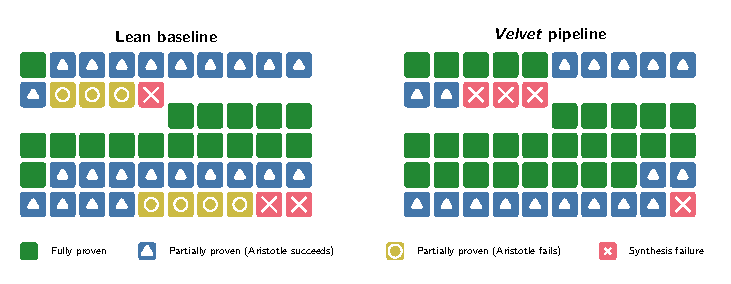
\includegraphics[width=0.88\textwidth]{assets/proof-waffle.pdf}

\end{frame}

\begin{frame}{Evaluation: RQ3 and RQ4}
\setlength{\parskip}{0pt}
\begin{columns}[T,onlytextwidth]
\begin{column}{0.46\textwidth}
{\large\textbf{\color{teal}RQ3: Closing the remaining proofs}}\par
\vspace{3mm}
Can additional proof effort close the remaining goals?\par
\vspace{4mm}
{\small Partially proven programs completed by Aristotle:\par}
\vspace{3mm}
\begin{tabular}{@{}l@{\hspace{8mm}}r@{}}
Lean & \textbf{23 / 30}\\[3mm]
Velvet & \textbf{\color{teal}18 / 18}
\end{tabular}
\vspace{5mm}

All partially proven Velvet programs were certified.\par
\end{column}
\begin{column}{0.46\textwidth}
{\large\textbf{\color{teal}RQ4: Across different LLMs}}\par
\vspace{3mm}
Does the advantage hold with another model?\par
\vspace{4mm}
{\small Fully proven programs at \$5 per problem:\par}
\vspace{3mm}
\begin{tabular}{@{}l@{\hspace{4mm}}r@{\hspace{4mm}}r@{}}
 & Lean & Velvet\\[2mm]
GPT-5.2 & 17/50 & \textbf{\color{teal}28/50}\\[3mm]
Opus 4.6 & 7/25 & \textbf{\color{teal}10/25}
\end{tabular}
\vspace{2mm}

{\footnotesize Opus: a random subset of 25 problems.\par}
\vspace{4mm}
Velvet leads under both models.\par
\end{column}
\end{columns}
\end{frame}

\begin{frame}{Summary}
\setlength{\parskip}{0pt}
\begin{columns}[T,onlytextwidth]
\begin{column}{0.47\textwidth}
\textbf{\color{teal}What have we seen}\par
\vspace{3mm}
\begin{itemize}
\setlength{\itemsep}{3mm}
\item<2-> \textbf{PBT is highly effective.}
\item<3-> \textbf{Decomposition simplifies synthesis.}
\item<4-> \textbf{Multi-modality pays off.}
\end{itemize}
\end{column}
\begin{column}{0.47\textwidth}
\uncover<5->{\textbf{\color{teal}Interesting future directions}}\par
\vspace{3mm}
\begin{itemize}
\setlength{\itemsep}{3mm}
\item<5-> \textbf{Certified synthesis of protocols and distributed systems.}
\item<6-> \textbf{Going Beyond functional correctness.}
\end{itemize}
\end{column}
\end{columns}

\vspace{6mm}
\uncover<7->{%
\centering
\textbf{Follow our work:} \href{https://verse-lab.org/}{verse-lab.org}\par
\vspace{2mm}
\href{https://github.com/verse-lab/velvet/}{Velvet}\quad$\cdot$\quad
\href{https://zenodo.org/records/22046794}{Artifact}\quad$\cdot$\quad
\href{https://verse-lab.org/papers/leetproof-ase26.pdf}{Paper}\par
\vspace{5mm}
{\large\textbf{\color{teal}Thank you!}\par}
}

\end{frame}

\end{document}
